\documentclass[11pt]{article}
\usepackage{outlines} %to do some fancy enumeration
\usepackage{titling} %to be able to drop or raise the title
\usepackage{amsmath} %for equations and symbols and such
\usepackage{cancel} %to cancel out terms in equations
%\usepackage{fullpage} %to make the margins smaller
\usepackage{geometry}
\geometry{letterpaper,portrait,margin=1in}
\usepackage{fancyhdr} %for headers and footers
\usepackage{graphicx}
\usepackage{float} %to put figures in certain spots
\usepackage{natbib} %for the bibliography
\usepackage{hyperref} %to be able to write web links
\usepackage{subfigure} %to put images side by side

\setlength{\droptitle}{-2cm}

\title{Charter School Competition: Evidence From Illinois Public Schools}
\author{NaLette Brodnax\\
\\
DRAFT: DO NOT CITE WITHOUT PERMISSION}
\date{STAT 626\\ December 11, 2014}

\begin{document}
\maketitle

\section{Executive Summary}
Over the past twenty years, charter schools have become an increasingly popular alternative to failing neighborhood schools.  Though they are publicly funded, charter schools are exempt from many of the state- and district-level policies governing structure, curriculum, personnel, and other aspects of learning.  Since the first charter school opened in 1992, over 4,000 charter schools have opened in forty states and the District of Columbia \citep{zimmer09}.

Charter schools face a tall order: in exchange for public funding and increased autonomy, they are expected to improve achievement and create competition for neighborhood schools, the administrations of which must adapt or face sanctions.  This analysis explores the extent to which traditional public schools (TPSs) respond to competition from charter schools.  Using data from Illinois public schools, I test whether proximity to a charter school is associated with an increase in aggregate achievement at the school level.  Using Bayesian estimation techniques, I find that charter school competition has a small, positive effect on the share of fourth grade students who meet or exceed the Illinois state standard for math achievement.

The remainder of this report is structured as follows.  Section two provides a brief review of recent studies on charter school competition.  Section three discusses the sources and construction of the data.  Section four comprises analyses of the data using exploratory graphics, linear regression, and hierarchical modeling.  Sections five and six discuss the findings and limitations of the analysis, respectively. 

\section{Literature Review}
Table 1 summarizes earlier studies' findings on the effects of charter school competition.  There are a number of challenges in comparing the results of the studies.  First, researchers measure competition in different ways.  Some consider competition to be the percentage of students transferring from TPSs to charter schools, referred to as the charter's market \textit{penetration}, while others measure a public school's \textit{proximity} to one or more charter schools. Second, researchers employ different units of analysis: six of the studies use school or district data, while the remaining use student data.  Finally, conclusions are mixed.  Early studies of charter school competition show positive effects on the achievement of traditional public schools, while more recent studies find no effects, negative effects, or small positive effects.  The mixed results may be attributed to several factors, such as state-level variation in charter school laws, local demography, or the political environment.

In order to avoid bias due to differences in state laws, I analyze charter school competition for just the state of Illinois.  Though student-level data is ideal, it is also the most difficult to acquire.  I use schools as the unit of analysis due to the ease of obtaining comprehensive data on school location, achievement, and characteristics.  I use proximity to the nearest charter school as the key measure of competition.  Proximity measures best capture the competitive effects that arise from charter schools' unique ability to enroll students from outside district boundaries.  Eight of the ten studies summarized in Table 1 feature proximity measures.

\begin{table}[h]
\caption{Summary of Competitive Effects on Traditional Public Schools}
  \centering
    \begin{tabular}{| l | l | l | l | l | c |}
    \hline
    Author(s) & State(s) & Year & Units & Measure & Effects \\ \hline
    Holmes et al. & NC & 2003 & Schools & Proximity & + \\
    Hoxby & MI,AZ & 2004 & Schools & Penetration & + \\ 
    Bohte & TX & 2004 & Districts & Both & + \\
    Bifulco \& Ladd & NC & 2004 & Students & Both & None \\
    Bettinger & MI & 2005 & Schools & Proximity & None \\
    Sass & FL & 2006 & Students & Both & + \\
    Booker & TX & 2008 & Students & Both & + \\ 
    Ni & MI & 2009 & Schools & Penetration & - \\
    Zimmer \& Buddin & CA & 2009 & Students & Both & None \\
    Kamienski & IL & 2011 & Schools & Proximity & None \\       
    \hline
    \end{tabular}
\end{table}

\nocite{hoxby04,holmes03,booker08,bohte04,bettinger05,bifulco04,kamienski11,sass06,ni09}

\section{Data}
The state of Illinois enacted charter school legislation in April 1996 and has since authorized over 100 charter schools, two-thirds of which are part of the Chicago Public Schools \citep{illinois_network_of_charter_schools_profiles_2012}.  Most charters are authorized by local school districts and governed by an independent board of directors.  Charter schools enroll 11\% of public school students in Chicago and 2.4\% of public school students statewide.  However, the Illinois Network of Charter Schools estimates that 15,000 students are on waiting lists for existing charters.

\paragraph{School Achievement Data} The Illinois State Board of Education publishes annual report card data\footnote{See \url{http://www.isbe.net/assessment/report_card.htm}}, including school-level assessment results for the Illinois State Achievement Test (ISAT).  The ISAT is administered to all students in grades third through eighth in math, reading, and science \citep{illinois_state_board_of_education_isbe_2009-2010_2012}.  Since most students learn to read by the end of third grade, I obtained the 2011 ISAT results in reading and math for all fourth grade students.  However, because the findings are similar for both subjects, this report provides only results related to math achievement.  ISAT performance is measured by the share of students who fall into one of four categories relative to the state standard: warning status, below standard, meets standard, or exceeds standard.  Throughout this report, I refer to the achievement rate as the share of students who meet or exceed the state standard.

The report card dataset also includes school characteristics, such as total enrollment, enrollment by race, student proportion receiving free or reduced lunch, student proportion with limited english proficiency, and student proportion receiving special education services.  The final dataset includes 1,685 elementary schools.

\paragraph{Proximity Data} As a measure of proximity, I use the shortest distance in miles between each school and the nearest charter school.  Note that distance is inversely related to proximity: as distance increases, proximity decreases.  To calculate the distance to the nearest charter school, I obtained latitude and longitude coordinates for each school from the National Center for Education Statistics\footnote{See \url{http://nces.ed.gov/ccd/elsi/tableGenerator.aspx}}.  The NCES data includes only the primary campus location for charter schools with multiple locations.  In order to incorporate all charter school campuses, I obtained the coordinates manually using the Bing Maps API and a web geocoding application\footnote{See \url{http://www.gpsvisualizer.com/geocoder/}}.

Figure 1 provides a map of traditional public schools and charter schools.  Most schools are concentrated in the upper right corner of the map, which is the Chicago metropolitan area.  However, there are a number of other clusters with charter schools around the state.

\begin{figure}[H]
\centering
    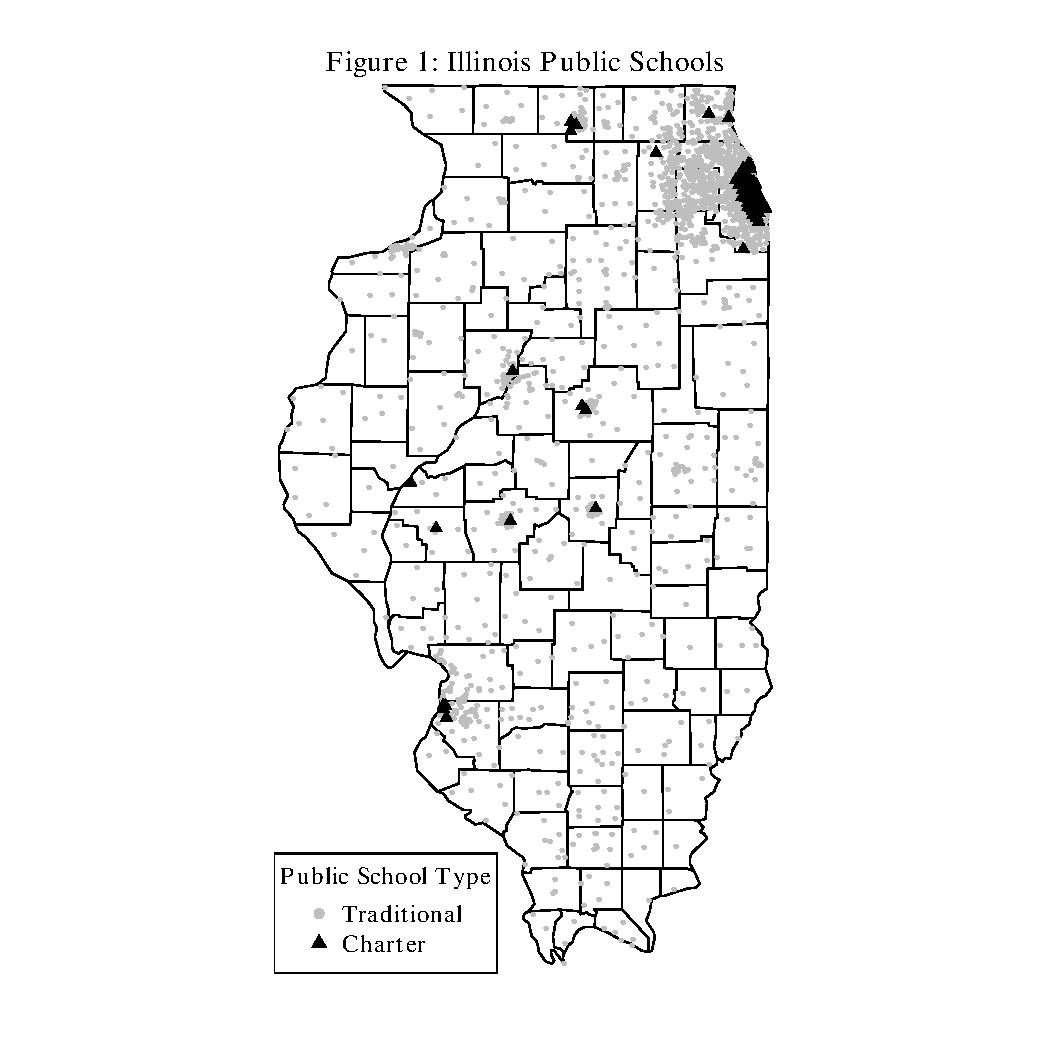
\includegraphics[trim=0 0.25in 0 0.25in, clip,scale=0.8]{ilmap}
        %trim={<left> <lower> <right> <upper>}
\end{figure}

\section{Analysis}

\subsection{Exploratory Analysis}
An exploratory graphical analysis of the data suggests that traditional public schools in close proximity to a charter school may have different achievement rates than schools located farther away.  Figures 2 shows the proportion of students meeting or exceeding the state standards for math in each school, plotted against the distance to the nearest charter school.  

\begin{figure}[H]
\centering
    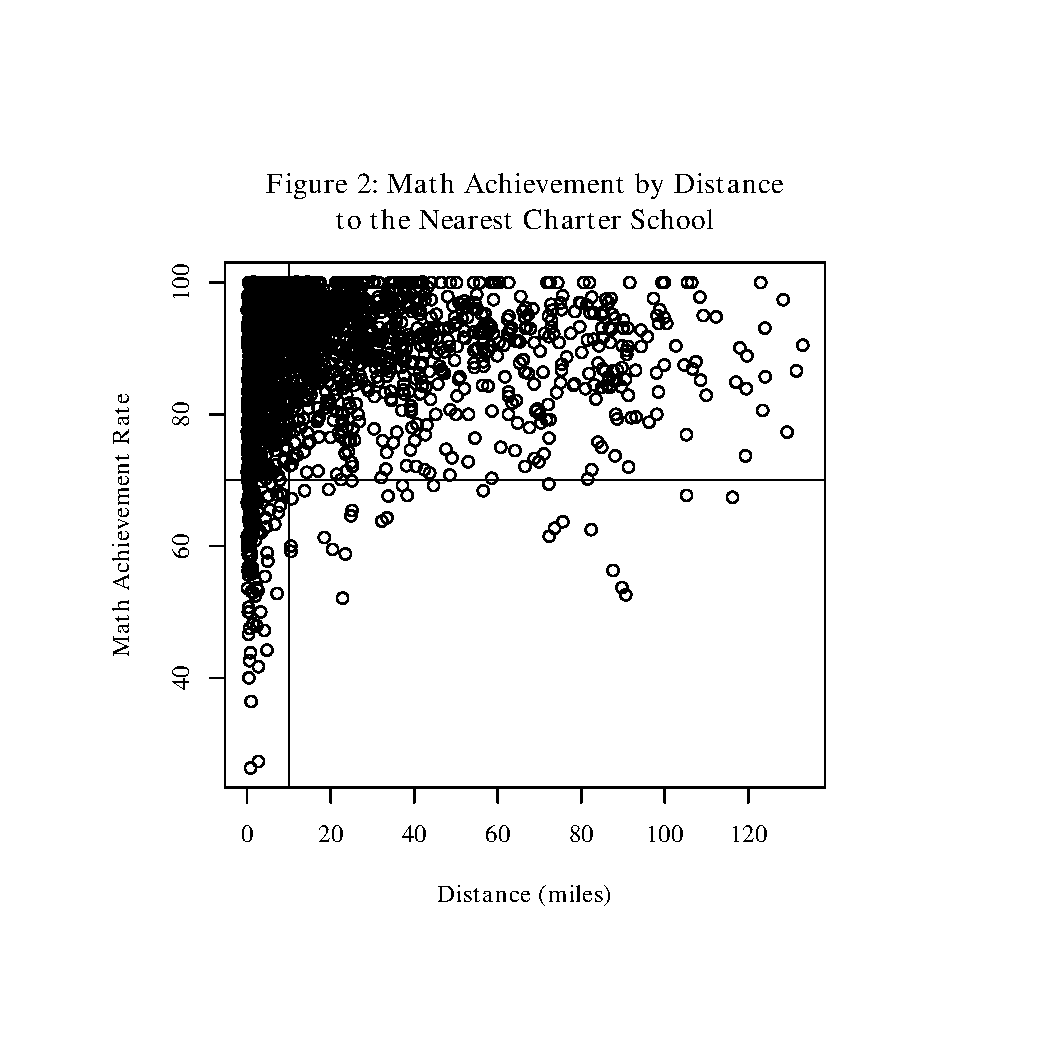
\includegraphics[trim= 0in 0.75in 0in 1in,clip,scale=0.8]{math_rate_dist}
    %trim={<left> <lower> <right> <upper>}
\end{figure}

Schools within a ten-mile radius of a charter school exhibit greater variation in their achievement rates.  For those schools with a math achievement rate higher than 80\%, the achievement rate appears to be randomly distributed without regard to distance.  However, schools with math achievement rates below 70\% appear to be clustered within a ten-mile radius of the nearest charter school.  The plots confirms what we already know: since charter schools are intended to be alternatives to failing schools, they tend to be located closest to the worst performing schools.  However, the relationship between distance and achievement is likely moderated by factors that are not apparent from a graphical review of the data.  Accounting for these factors is the topic of the next section.

\subsection{Empirical Method: Linear Regression}
Linear regression is a powerful technique used to estimate the relationship between two variables.  Assuming that the relationship between achievement and distance to a charter school is linear, the achievement rate can be represented by the following model:
\begin{equation*}
Y_i=\beta_0+\beta_1X_i+\epsilon
\end{equation*}
where $Y_i$ is the \textit{achievement rate}, defined as the proportion of students in school $i$ meeting or exceeding the state math standard on the ISAT, and $X_i$ is the shortest distance to the nearest charter school.  If proximity to a charter school has a positive effect on TPS achievement, then I expect to see a negative coefficient for $\beta_1(distance)$.

Achievement is influenced by a variety of factors related to school practices and student characteristics.  To control for these observed characteristics, I include a number of covariates that are known to explain achievement outcomes.  First, achievement is strongly correlated with the racial and socioeconomic composition of a school, as low-performing schools tend to have high concentrations of poor students and racial minorities \citep{orfield_why_2005,gamoran_equality_2006,jencks_black-white_1998}.  Second, students with limited English skills score lower than their peers on achievement tests and are concentrated in poor schools \citep{reardon_s.f._hispanic-white_2009,orfield_why_2005}.  Finally, achievement may be influenced by the surrounding neighborhood, which may be in a densely populated urban area or in a rural area.  To account for these factors, I include school-level measures for the proportion of black students in the school, the proportion of students with limited English proficiency, the proportion of students receiving free or reduced lunch, and total enrollment.  Descriptive statistics for all variables are given in Table 2.  

\begin{table}[h]
\centering
\caption{Descriptive Statistics} 
\begin{tabular}{|l|c|c|c|c|}
  \hline
 & Mean & S.D. & Min & Max \\ 
  \hline
Achievement Rate & 86.807 & 11.162 & 26.3 & 100.0 \\ 
   \hline
Proximity & 22.901 & 26.503 & 0.003 & 133.062 \\ 
   \hline
Pct Black & 21.357 & 33.059 & 0.0 & 100.0 \\ 
   \hline
Enrollment & 395.161 & 200.666 & 29.0 & 1071.0 \\ 
   \hline
Pct English Learners & 9.677 & 15.126 & 0.000 & 70.0 \\ 
   \hline
Pct Low Income & 54.809 & 31.114 & 0.20 & 100.0 \\ 
   \hline
N = 1685 &  &  &  &  \\ 
   \hline
\end{tabular}
\end{table}

Regression coefficients, $\beta_j$ are typically estimated by minimizing the sum of the squared residuals, a technique known as Ordinary Least Squares.  These coefficients can also be estimated with a Bayesian approach: given a sampling model for the data and a set of prior beliefs, posterior beliefs can be approximated via Bayes Theorem.  Applied to the regression case, the posterior distribution of $\beta$ is
\begin{equation*}
p(\beta\vert\ y,X,\sigma^2) \propto p(y\vert X,\beta,\sigma^2)\times p(\beta).   
\end{equation*}

I assume that the sampling model for $y$ has a multivariate normal form, the prior distribution of $\beta$ has a conjugate multivariate normal form, and the prior distribution of $\phi=1/\sigma^2$ has a semi-conjugate gamma form, which give the following posterior distributions:
\begin{align*}
& p(\beta\vert y,X,\sigma^2)\propto exp\bigg[\beta^T\bigg(\Sigma_0^{-1}\beta_0+\frac{X^Ty}{\sigma^2}\bigg)-\frac{1}{2}\beta^T\bigg(\frac{\Sigma_0^{-1}+X^TX}{\sigma^2}\bigg)\beta\bigg]\\
& p(\phi\vert y,X,\beta) \propto \phi^{(\nu_0+n)/2-1}exp\big(-\phi\big[\nu_0\sigma_0^2+\text{SSR}(\beta)\big]/2\big)
\end{align*}

My specification of prior parameters is simplified by using Zellner's g-prior \citep{hoff09}.  Zellner's g-prior stabilizes parameter estimates, prevents model overfitting, and allows posterior approximation via Monte Carlo sampling.  Using achievement data from 2009, I set $\sigma_0^2=\sigma_{ols}^2$ and $g=n=1685$, with a weakly-informative prior sample size of $\nu_0=1$.  Estimation results are given in Table 3.

\begin{table}[h]
\centering
\caption{Bayesian Estimation Results for $\mathbf{\beta_j}$} 
\begin{tabular}{|l|c|c|}
  \hline
 & $\beta_j$ & 95\% Confidence Region \\ 
  \hline
Intercept & 99.569 & 98.174 $<\beta_0<$ 101.003 \\ 
   \hline
Proximity & -0.031 & -0.050 $<\beta_1<$ -0.013 \\ 
   \hline
Pct Black & -0.087 & -0.109 $<\beta_2<$ -0.065 \\ 
   \hline
Enrollment & 0.000 & -0.002 $<\beta_3<$ 0.003 \\ 
   \hline
Pct English Learners & -0.097 & -0.138 $<\beta_4<$ -0.058 \\ 
   \hline
Pct Low Income & -0.172 & -0.193 $<\beta_5$ -0.149 \\ 
   \hline
\end{tabular}
\end{table}

Accounting for other factors that influence achievement, the coefficient for distance is small and negative.  In other words, the smaller the distance between a traditional public school and the nearest charter school (and the greater the proximity), the higher the achievement.  The 95\% confidence region for $\beta_1(distance)$ does not contain zero, so I conclude that proximity has a small, positive effect on achievement.  Figure 3 provides a plot of the posterior $\beta$ samples generated using Monte Carlo sampling.  The samples in gray show that there is considerable uncertainty in the estimates, particularly for distances greater than 60 miles, where the sample of schools is much smaller.  Despite this uncertainty, all samples show a negative relationship between distance and achievement.

\begin{figure}[H]
\centering
    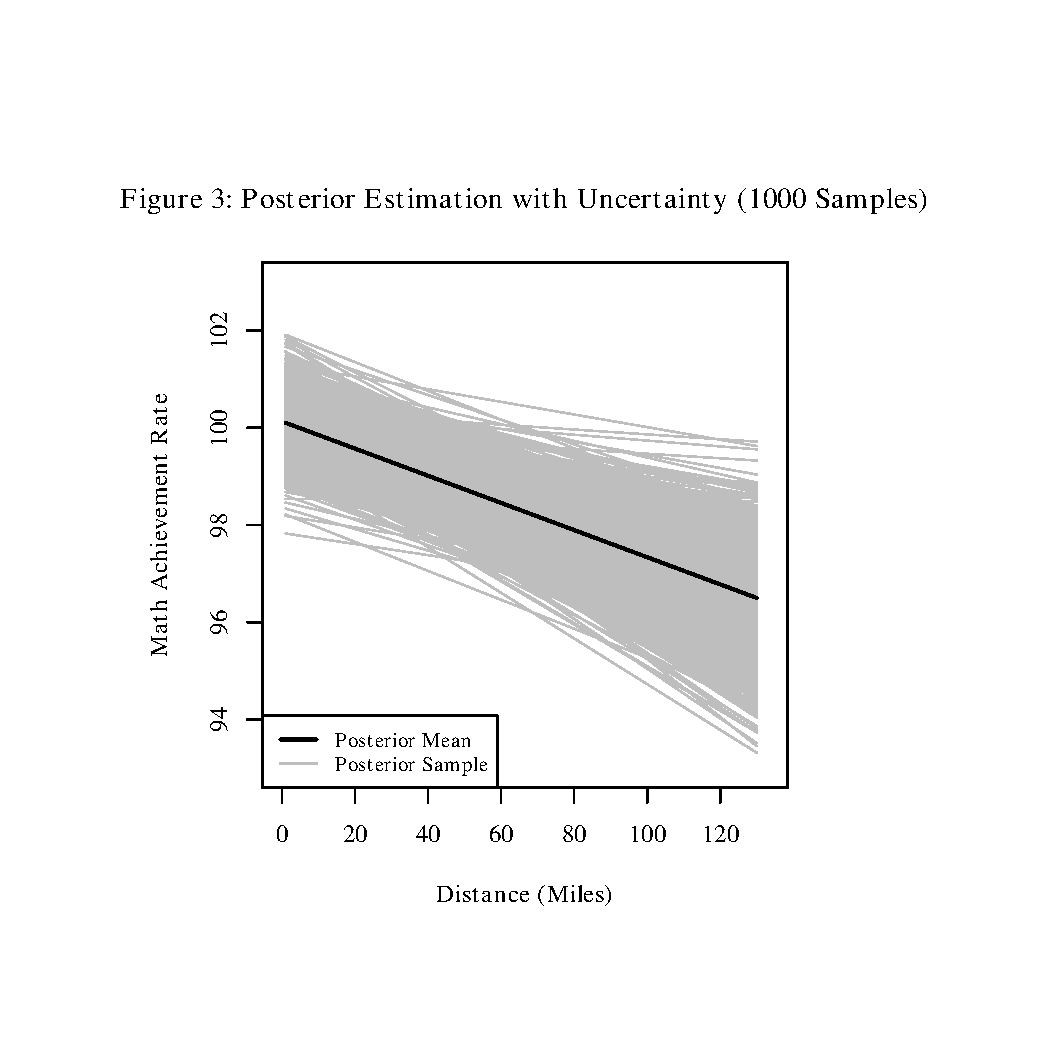
\includegraphics[trim= 0in 0in 0in 1in,clip,scale=0.8]{post_lines}
    %trim={<left> <lower> <right> <upper>}
\end{figure}

The implication that proximity to a charter school results in higher achievement contradicts the exploratory analysis, which seemed to show higher achievement with larger distances.  The regression results demonstrate the importance of controlling for confounding factors, such as racial composition, the proportion of students with limited English proficiency, and the proportion of students in low-income households.  However, the linear regression model does not address the spatial structure of the data.  The next section considers ways to account for spatial clustering of schools.

\subsection{Cluster Analysis: Hierarchical Modeling}
A review of the map of Illinois in Figure 1 shows that neither public schools nor charter schools are randomly distributed; rather, they are clustered within counties and districts.  Since charter schools are not required to adhere to district boundaries, a district-level analysis may be too noisy.  However, most of the geographic clusters appear to be located in distinct counties.  

Figure 4 provides box plots of the math achievement rate for all 101 counties containing elementary schools.  The mean achievement rate of 89\% for all schools is represented by the horizontal bar.  Two issues are apparent.  First, there is considerable variation between counties, as shown by the locations of the means in each box plot in comparison to the mean for all schools.  Second, there is variation within districts, as the individual county boxes are different sizes.

\begin{figure}[H]
\centering
    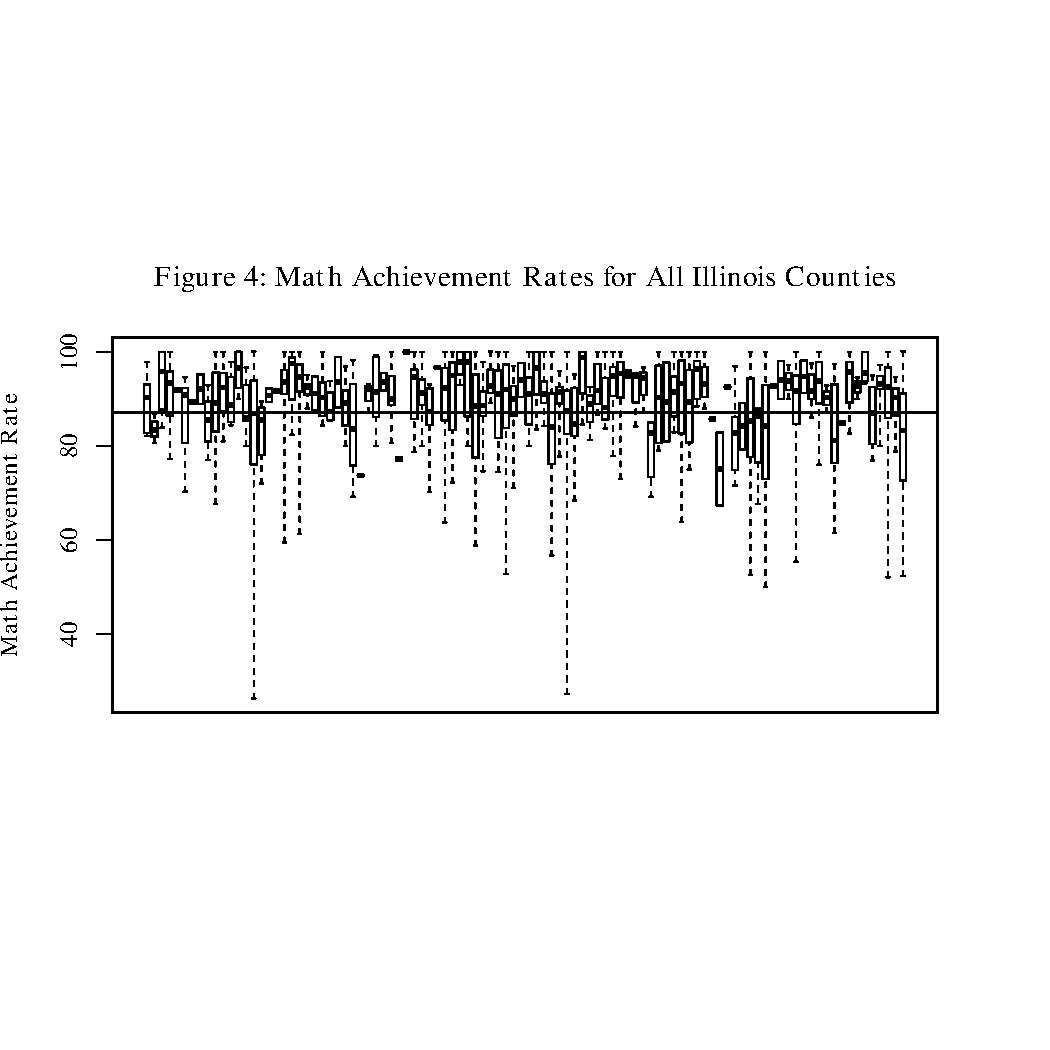
\includegraphics[trim= 0in 2in 0in 1.75in,clip,scale=0.8]{counties}
    %trim={<left> <lower> <right> <upper>}
\end{figure}

In order to determine the extent to which achievement is influenced by school factors relative to district factors, I estimate the achievement rate using a hierarchical normal model.  Given $n=1685$ schools clustered in $m=101$ counties\footnote{There are 102 counties in Illinois.  For future analyses, I intend to investigate which county is missing and assess the impact of the missing data on analysis outcomes.} and a normally distributed sampling model, Gibbs sampling can be used to approximate the posterior distributions from the full conditional distributions of four key parameters: 
\begin{enumerate}
\item The mean achievement rate for each county, $\theta_1,...,\theta_m\sim \text{normal}(\mu,\tau^2)$;
\item The mean achievement rate of the population of counties, $\mu\sim\text{normal}(\mu_0,\gamma_0^2)$;
\item The variance for the population of counties (between-group variation), \\$\tau^2\sim\text{inverse-gamma}(\eta_0/2,\eta_0\tau_0^2/2)$;
\item The variance for each sample of schools (within-group variation), \\$\sigma^2\sim\text{inverse-gamma}(\nu_0/2,\nu_0\sigma_0^2/)2$ 
\end{enumerate}

I implemented the Gibbs sampler with 5,000 iterations, using the mean and variance of the 2009 achievement rates as prior starting points: $\mu_0=84.7$ and $\sigma_0^2=\tau_0^2=169.2$.  I set the population variance prior $\gamma_0^2=25$ in order to cap the upper bound of the achievement rate at 100.  Prior sample sizes reflect a high degree of uncertainty at $\eta_0=\nu_0=2$.  The posterior achievement rates for all counties are shown in Figure 5 with a line for the posterior mean of 89.6\%.  The distribution of the posterior samples is consistent with the degree of variation shown across counties in Figure 4.  The posterior mean is $\approx 3$ percentage points higher than the mean achievement rate in the 2011 data, despite a prior (but weakly informative) rate of 84.6\%.

\begin{figure}[H]
\centering
    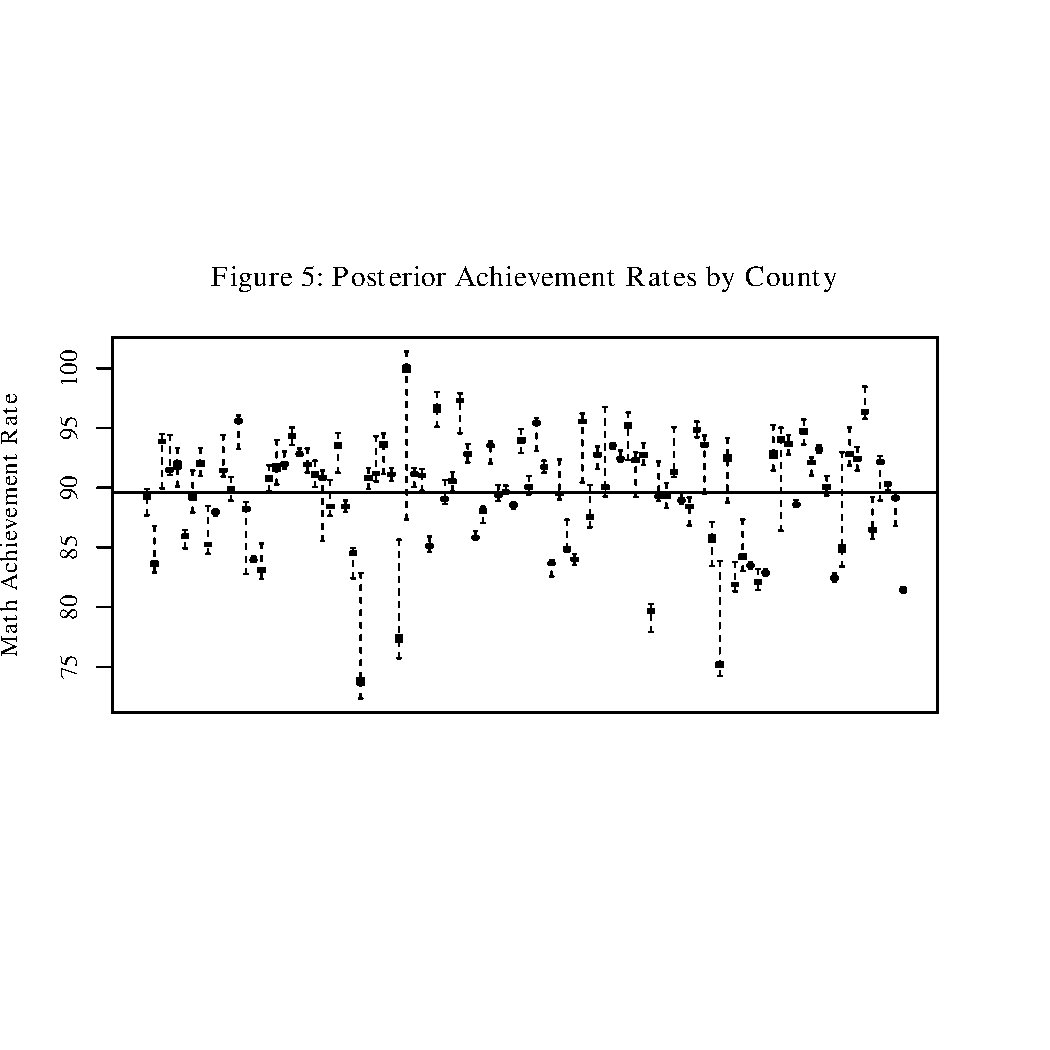
\includegraphics[trim= 0in 2in 0in 1.75in,clip,scale=0.8]{theta_post}
    %trim={<left> <lower> <right> <upper>}
\end{figure}

\paragraph{Gibbs Sampler Convergence} In order to check whether there were any problems with the Gibbs sampler, I compute effective sample sizes and review stationarity plots to check for convergence.  The stationarity plots for the posterior samples of $\mu, \tau^2$, and $\sigma^2$ are shown below.  All samples have converged well before the 5,000th iteration.  Effective sample sizes for $\mu, \tau^2$, and $\sigma^2$ are sufficiently large, at 5,000, 4,433, and 5,000, respectively.  The effective sample sizes for $\theta_1,...,\theta_m$ are also sufficiently large, ranging from 4,469 to 5,000.

\begin{figure}[H]
\centering
    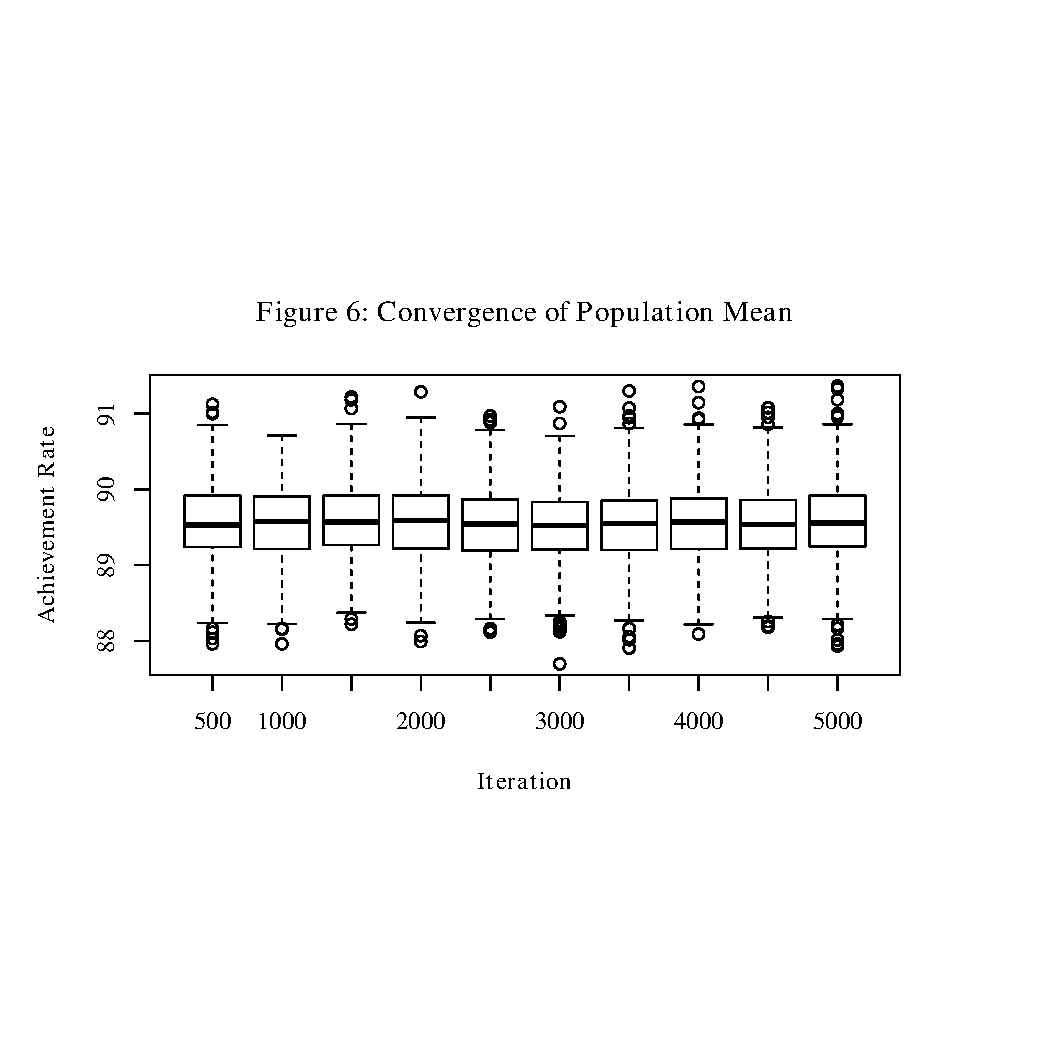
\includegraphics[trim= 0in 1.5in 0in 1.5in,clip,scale=0.8]{mu}
    %trim={<left> <lower> <right> <upper>}
\end{figure}
\begin{figure}[H]
\centering
    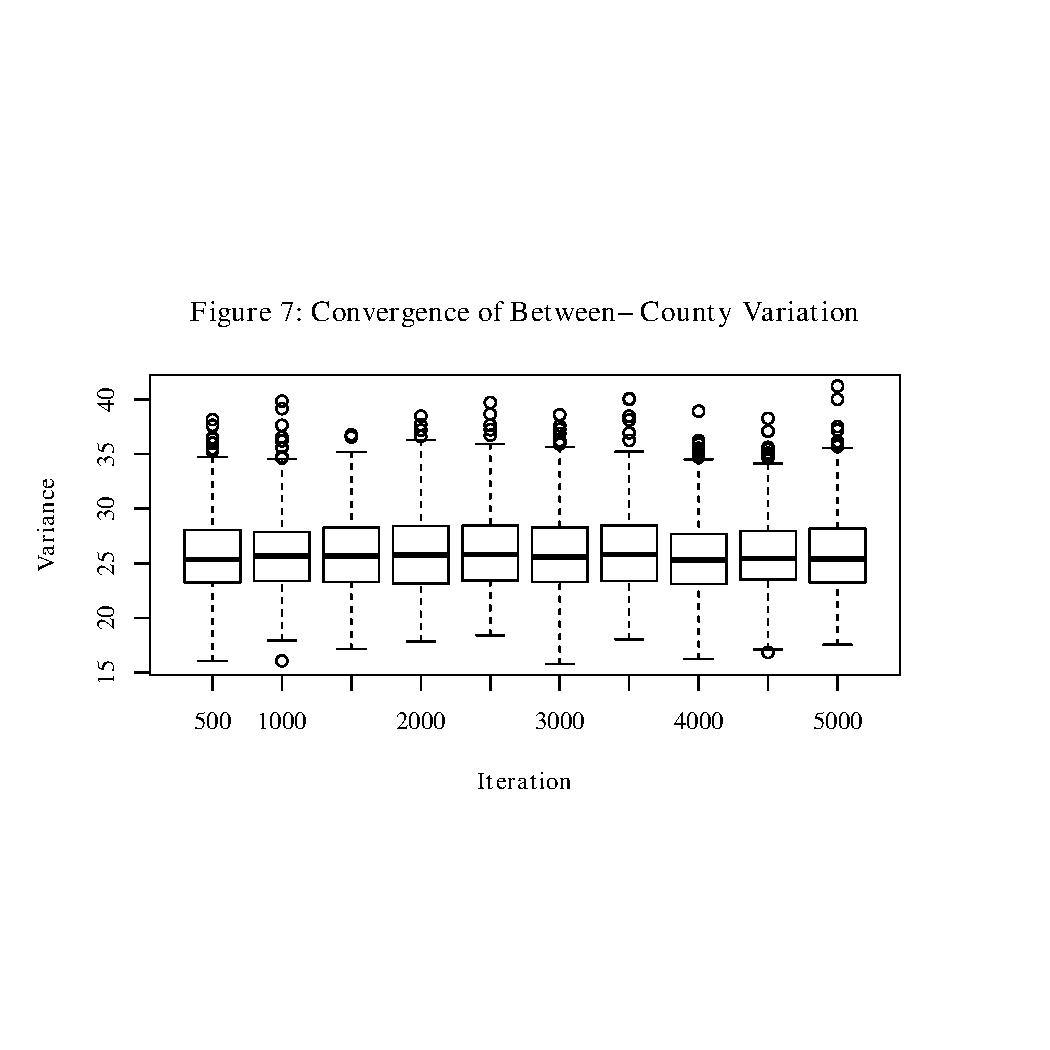
\includegraphics[trim= 0in 1.5in 0in 2in,clip,scale=0.8]{tau}
    %trim={<left> <lower> <right> <upper>}
\end{figure}
\begin{figure}[H]
\centering
    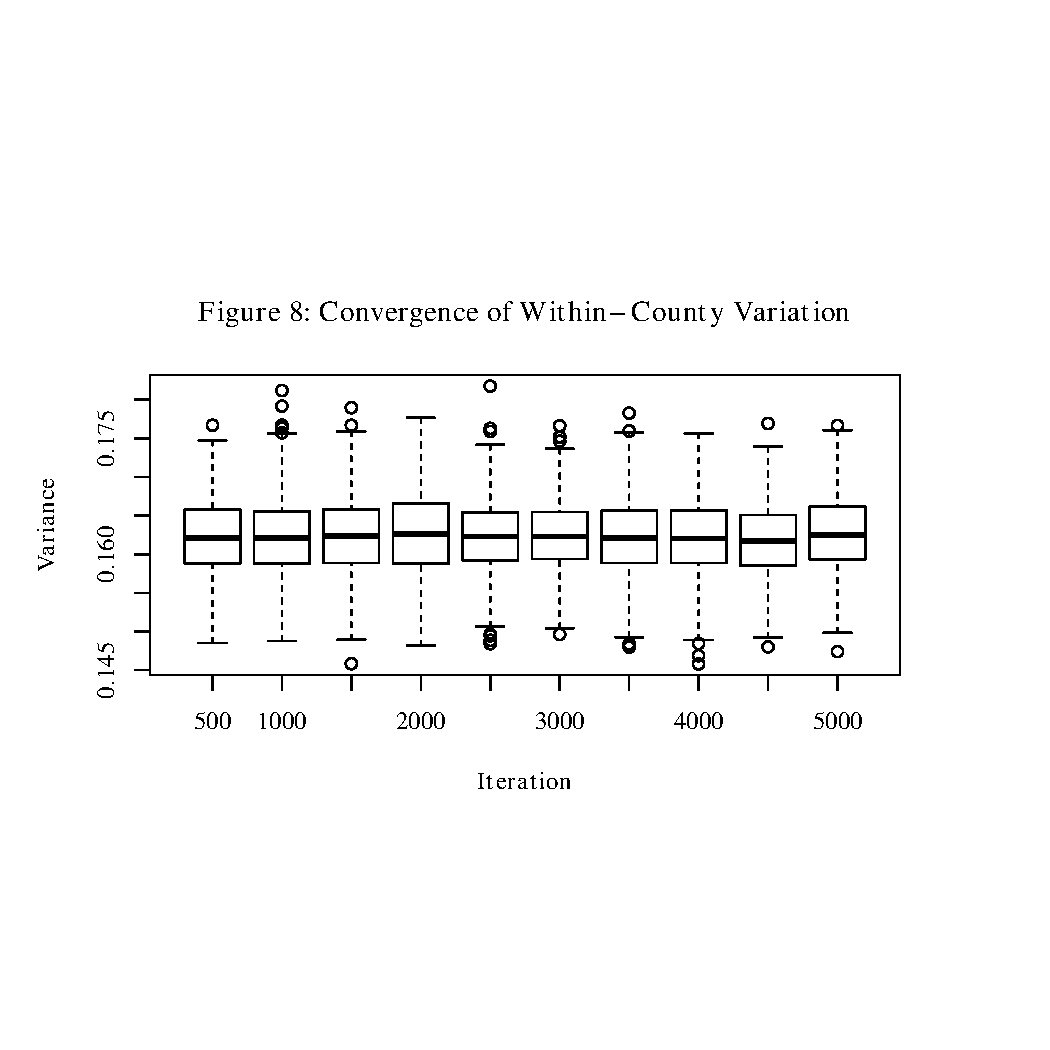
\includegraphics[trim= 0in 1.5in 0in 2in,clip,scale=0.8]{sigma}
    %trim={<left> <lower> <right> <upper>}
\end{figure}

\paragraph{Posterior Inference}  The parameter $\mu$ is a ``hyper-parameter" for the mean of the population of counties.  Its posterior mean $E[\mu\vert\theta_1,...,\theta_m,\tau^2]$ is 89.55, with a 95\% confidence region between 88.53 and 90.52.  The posterior and prior densities of the mean achievement rate are shown in Figure 9 below.  In comparison to the prior, the posterior density has a higher mean and much smaller variance.  

\begin{figure}[H]
\centering
    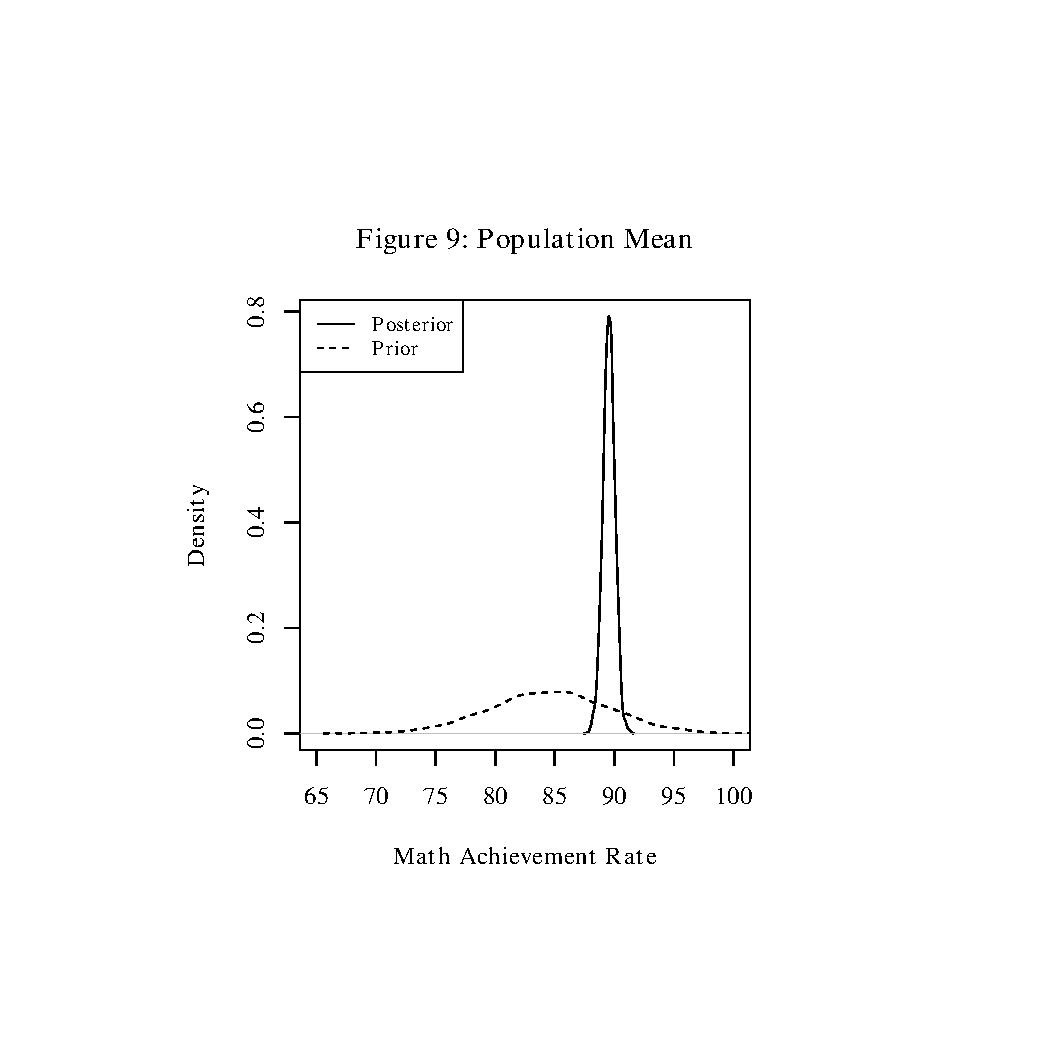
\includegraphics[trim= 0in 1in 0in 1.5in,clip,scale=0.8]{mu_post}
    %trim={<left> <lower> <right> <upper>}
\end{figure}

The parameter $\tau^2$ is also a hyper-parameter for the variance of the population of counties.  It is commonly referred to as \textit{between-group} variation.  The posterior mean for $\tau^2\vert\theta_1,...,\theta_m,\mu$ is 25.91, with a 95\% confidence region between 19.64 and 34.22.  This means that 95\% of the county means will fall within $\approx 5$ percentage points of the population mean--a substantively large amount of variation.  A comparison of the posterior and prior densities of $\tau^2$ is given in Figure 10.
  
The parameter $\sigma^2$ is the variation between individual schools within a given county, commonly referred to as \textit{within-group} variation\footnote{For the purpose of this analysis, I assume that $\sigma^2$ is constant.  However, this is a strong assumption given the within-county variation that is present in Figure 4.  It is possible to specify a hierarchical model that allows $\sigma^2$ to vary by school.}.   The posterior mean for $\sigma^2\vert\theta_1,...,\theta_m,y_1,...y_m$ is 0.162 and the 95\% confidence region is between 0.152 and 0.172).  In comparison to the between-group variation, within-group variation is much smaller.  The posterior and prior densities of $\sigma^2$ are given in  Figure 11.
\begin{figure}[H]
\hfill
\subfigure{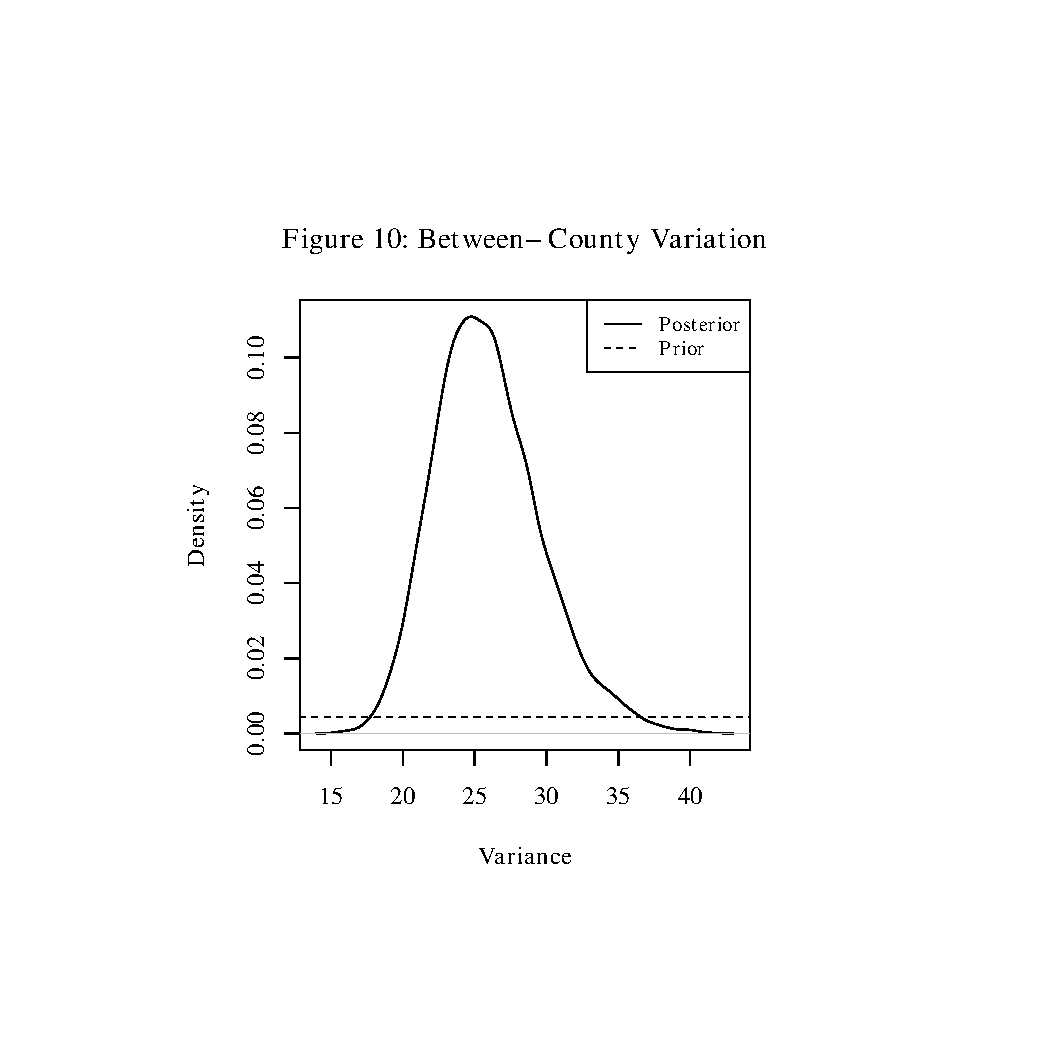
\includegraphics[trim= 1.25in 1in 1.9in 1.5in,clip,width=3in]{tau_post}}
\hfill
\subfigure{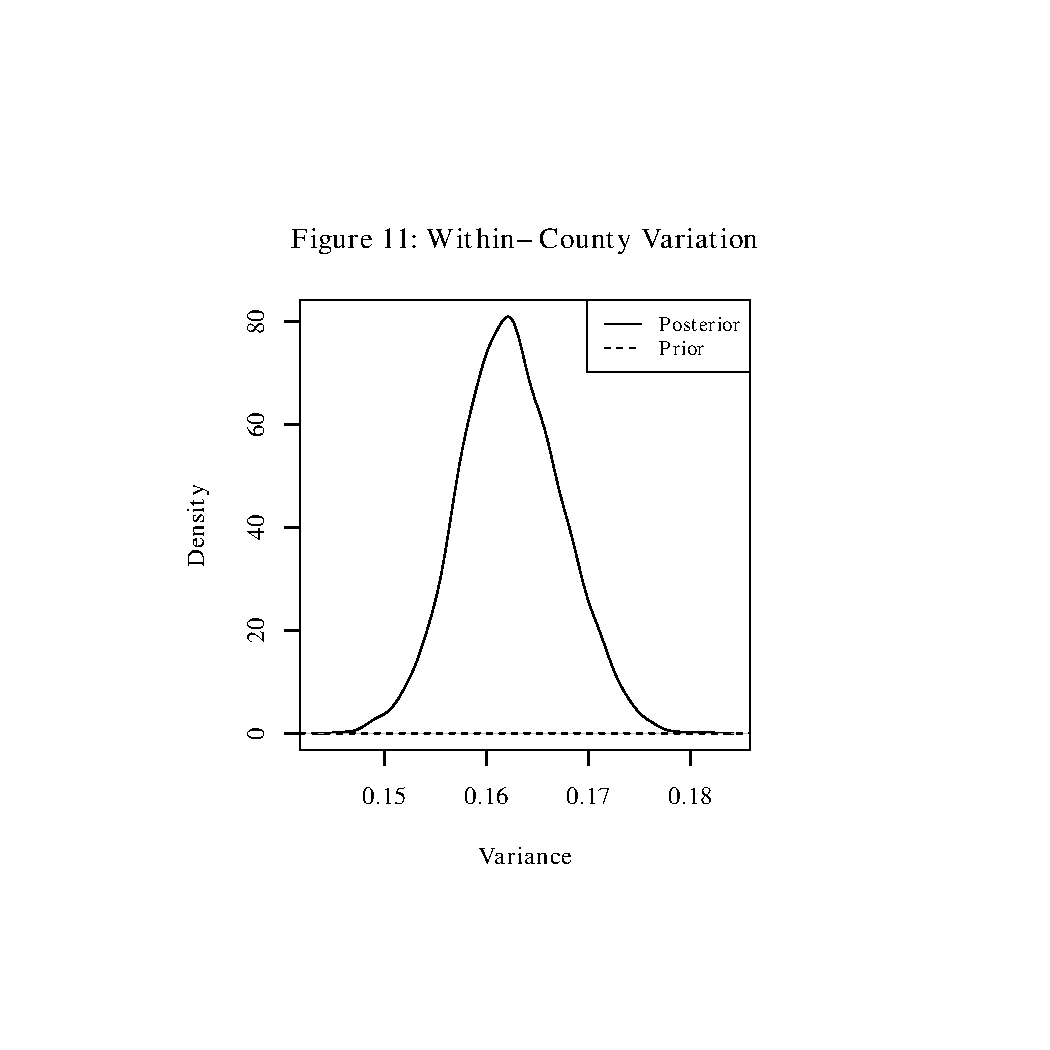
\includegraphics[trim= 1.25in 1in 1.9in 1.5in,clip,width=3in]{sigma_post}}
\hfill
\end{figure}

\section{Findings and Implications}
This study aims to test the relationship between school-level achievement and proximity to a charter school, resulting in three key takeaways.  First, the linear regression results provide evidence that proximity to a charter school has a small, positive effect on a traditional public school's math achievement rate.  The coefficient on the proxy for proximity, \textit{distance}, is -0.031: the farther away the nearest charter school, the lower the achievement rate.

Second, math achievement is strongly correlated with student characteristics.  The coefficients in the regression model for the proportion of black students, the proportion of students with limited English proficiency, and the proportion of students in low-income households are all negative and significant, at -0.087, -0.097, and -0.172, respectively.  The negative effect of having a larger proportion of low-income students is more than five times the positive effect of being located near a charter school.  

Third, the cluster analysis via hierarchical modeling demonstrates a strong relationship between location and achievement.  Variation in achievement rate is much larger between counties than between schools within counties.

The findings of this analysis are relevant for policymakers who continue to champion charter schools as beneficial for students.  The results of this study suggest that when charter schools open in a neighborhood, even students who do not attend the charter school may benefit from its presence.  However, additional work is needed to better estimate the effect of charter school proximity on traditional public schools.

\section{Limitations}
Statistician George E. P. Box remarked that, ``Essentially, all models are wrong, but some are useful" \citep{box87}.  While I find the results of this analysis useful for policymakers and education practitioners, the comments below highlight aspects of the models that are known to be `wrong' and suggest ways to improve them.
\begin{enumerate}
\item \textbf{Lack of Causal Inferences} This study relies on observational data and therefore does not feature a precise treatment and counterfactual group on which to base causal inferences.  Though covariates are included in the regression model, these do not account for unobserved differences between schools which may confound the effect of being located near a charter school.  One way to reduce bias would be to obtain achievement data for numerous years and use a fixed-effect specification to control for unobserved, time-invariant factors.
\item \textbf{Poorly Fit Sampling Model} For the regression and hierarchical models, I assumed that school achievement rates are normally distributed.  While the normality assumptions allows ease of computation, achievement rates may be better fit by a different distribution.  Since the achievement rate is always a share of the total student population, it may not conform to a normal distribution.  \cite{ferrari04} recommend beta regression for parameters that are continuous and bound to the interval (0,1), such as proportions.  While they advocate maximum likelihood estimation for parameters, I would investigate ways to use beta regression within a Bayesian framework.
\item \textbf{Inadequate Hierarchical Structure}  This analysis attempted to explicitly model the spatial structure of the data in order to consider the impact of this structure on estimation results.  However, there are two issues with this approach.  First, the hierarchical model includes only two levels: counties and schools.  A more comprehensive model might include an additional level for school district or neighborhood.  Second, the hierarchical model lacks controls for confounding factors at the school level.  The hierarchical model can be adapted to a regression framework so that additional information can be incorporated at each level \citep{hoff09}.
\end{enumerate}
In conclusion, this analysis makes an important contribution to the debates about the role of charter schools in education reform.  Future studies should address not only the limitations of this analysis, but also the degree to which the results can be generalized to other settings. 

\newpage
\bibliographystyle{apa}
\bibliography{/Users/nbrodnax/Research/Projects/endnote,/Users/nbrodnax/Research/Projects/zotero}{}


\end{document}
